\section{Graph 3-coloring Problem}

% First idea: Generate all bonds with colored atoms and verify the entire system (haha, complexity like $O(n^4)$ because $|E| \in O(n^2) $). Second solution: Generate a reverse-order sequence of vertices and let it order in the correct order. All pairs should meet each other, the problem to solve is whether all pairs really meet each other. After that verify that the area is full like Winfree -- from one side to the other. Improvement: the verification can be triggered from both sides simultaneously.

% Remind original Knuth's algorithm at \url{http://www.iti.fh-flensburg.de/lang/algorithmen/sortieren/networks/oetsen.htm}! And prove that everything goes fine! Robusticity? %!% citovat někde

Another $\NPC$ problem is Graph 3-coloring Problem, its task is to decide whether there exists an assignment of three colors to vertices of the graph so that no connected vertices have the same color.

If $k$ is odd, we add a separated vertex thus resulting graph $G'$ is 3-colorable if and only if original graph $G$ is 3-colorable. See example in Figure \ref{fig:3-color}.

%!% přidat převod na SAT (myslim že n log n) ?

% Note that there exists a reduction of $\sf SAT$ in Cunjunctive Normal Form with length $n$ to Graph 3-coloring Problem on $O(n\log n)$ vertices.   %!% když už tak všude ty převody

\subsection*{Set of tiles}

\begin{description}
	\item[Bottom tiles.] These tiles have colorless labels $2l$ and $2l-2$ $(0 < l \leq \frac{k}{2})$ on the bottom left and right sides, respectively. On the top sides there are all color combinations of $2l-1$ and $2l-2$; if corresponding vertices are connected by edge, single-color combinations can be omitted. $\frac{9n}{2}$ tile types were required.
	\item[Bottom corner tiles.] These tiles are exactly the same like for $k$-clique. $2$ tile types were required.
	\item[Inner tiles.] These tiles are responsible for numerical ordering, they are very similar to those in previous problem. There exist all color combinations for all different numbers in both orders on the bottom sides with an exception: there do not exist tiles with numbers of connected vertices with the same color. Thus as soon as there meet vertices which are connected and have the same color, the assembly stops. Moreover there exist similar tiles with sharp and asterisk with an exception: sharp and the least number, and largest number and asterisk do not exist because they will trigger verification. $\binom{n}{2} \cdot 2 \cdot 9 + 2 \cdot 3 (n-1) - 2 \cdot 3 e \sim 9n^2 - 6e$ tile types were required.
	\item[Border tiles.] These tiles are exactly the same like for $k$-clique. $2$ tile types were required.
	\item[Verification tiles.] These tiles are almost the same like for $k$-clique, the only difference is that they are triggered by the least and the largest number instead of the least and the largest color, respectively. $3n$ tile types were required.
	\item[DONE tile.] The tile is exactly the same like for $k$-clique. $1$ tile type was required.
\end{description}

Summed up, tile complexity of this DNA algorithm is asymptotically equivalent to $9n^2 - 6e$. Binding complexity is asymptotically equivalent to $\nicefrac{5}{4}\,n^2$, glue complexity is asymptotically equivalent to $\nicefrac{7}{2}\,n$.

\begin{figure}[H]
\begin{center}
	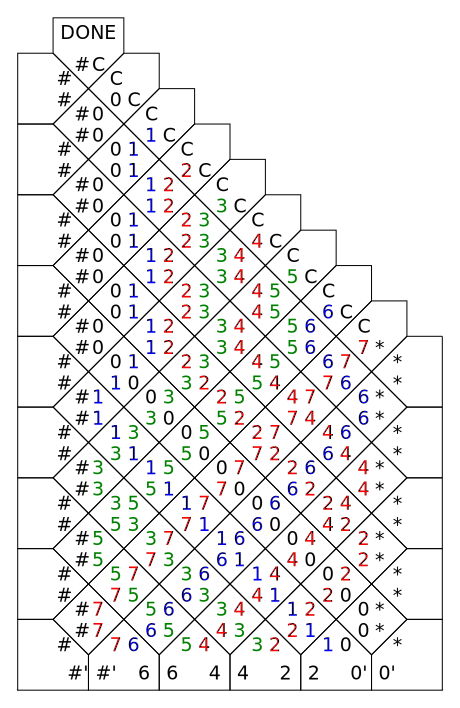
\includegraphics[scale=0.75]{./figures/3-color/3-color.pdf}
	\caption{3-color computation.}
	\label{fig:3-color}
\end{center}
\end{figure}
